\documentclass[11pt]{beamer}
\usetheme{Boadilla}
\usepackage[utf8]{inputenc}
\usepackage{amsmath}
\usepackage{amsfonts}
\usepackage{amssymb}
\usepackage{tikz}
\usepackage{float}
\usepackage{graphicx}
\usetikzlibrary{calc,trees,positioning,arrows,chains,shapes.geometric,%
    decorations.pathreplacing,decorations.pathmorphing,shapes,%
    matrix,shapes.symbols}

\tikzstyle{punktchain} = [rectangle, 
    rounded corners, 
    draw=black, very thick,
    text width=10em, 
    minimum height=3em, 
    text centered, 
    on chain,
    top color=white, 
    bottom color=blue!20]
\tikzstyle{arrow} = [thick,->,>=stealth]
\author{Erik Thorsen}
\title{Anomaly detection in NGS quality control data}
%\setbeamercovered{transparent} 
%\setbeamertemplate{navigation symbols}{} 
%\logo{} 
%\institute{} 
%\date{} 
%\subject{} 
\begin{document}

\begin{frame}
\titlepage
\end{frame}

%\begin{frame}
%\tableofcontents
%\end{frame}

\begin{frame}{Problem description}
\begin{itemize}
\item Detect anomalies based on quality control data from NGS machines.
\item What is a anomaly/what are we looking for? Transient behaviours (poor samples on flowcells/poor preparation), trends (is a machine starting to break or new maintenance routine). If new trends are showing $\rightarrow$ estimate when the change started?
\item Construct a model of some sort which can monitor the machine (unsupervised).
\end{itemize}
Next some exploratory data analysis.
\end{frame}

\begin{frame}{Exploratory data analysis}{No. of flowcells (runs) stratified on each completed cycle}
\begin{table}[ht]
\centering
\begin{tabular}{llllllllll}
  \hline
cycles & Hi3 & Hi4 & Hi5 & Hi6 & HiX1 & HiX2 & HiX3 & HiX4 & HiX5 \\ 
  \hline
49 & 7 &  &  &  &  &  &  &  &  \\ 
  50 & 16 & 10 & 11 & 7 &  &  &  &  &  \\ 
  60 &  &  &  & 3 &  &  &  &  &  \\ 
  99 & 2 & 4 & 2 & 1 &  &  &  &  &  \\ 
  100 & 73 & 49 & 15 & 6 &  &  &  &  &  \\ 
  124 &  & 22 & 22 & $\mathbf{30}$ &  &  &  &  &  \\ 
  125 &  & 53 & 46 & $\mathbf{50}$ &  &  &  &  &  \\ 
  150 & 11 & 2 & 14 & 16 & 30 & 27 & 22 & 32 & 16 \\ 
  200 &  &  &  & 1 &  &  &  &  &  \\ 
  250 & 6 & 1 &  &  &  &  &  &  &  \\ 
  \hline
  $\Sigma$ & 115 & 141 & 110 & 114 & 30 & 27 & 22 & 32 & 16 \\ 
   \hline
\end{tabular}
\caption{Table showing the number of completed cycles for each HiSeq (Hi) and HiSeqX (HiX) machine.} 
\label{CompCycl}
\end{table}
\end{frame}

\begin{frame}{Exploratory data analysis}{Tag level - mean q values for each flowcell} 
\begin{center}
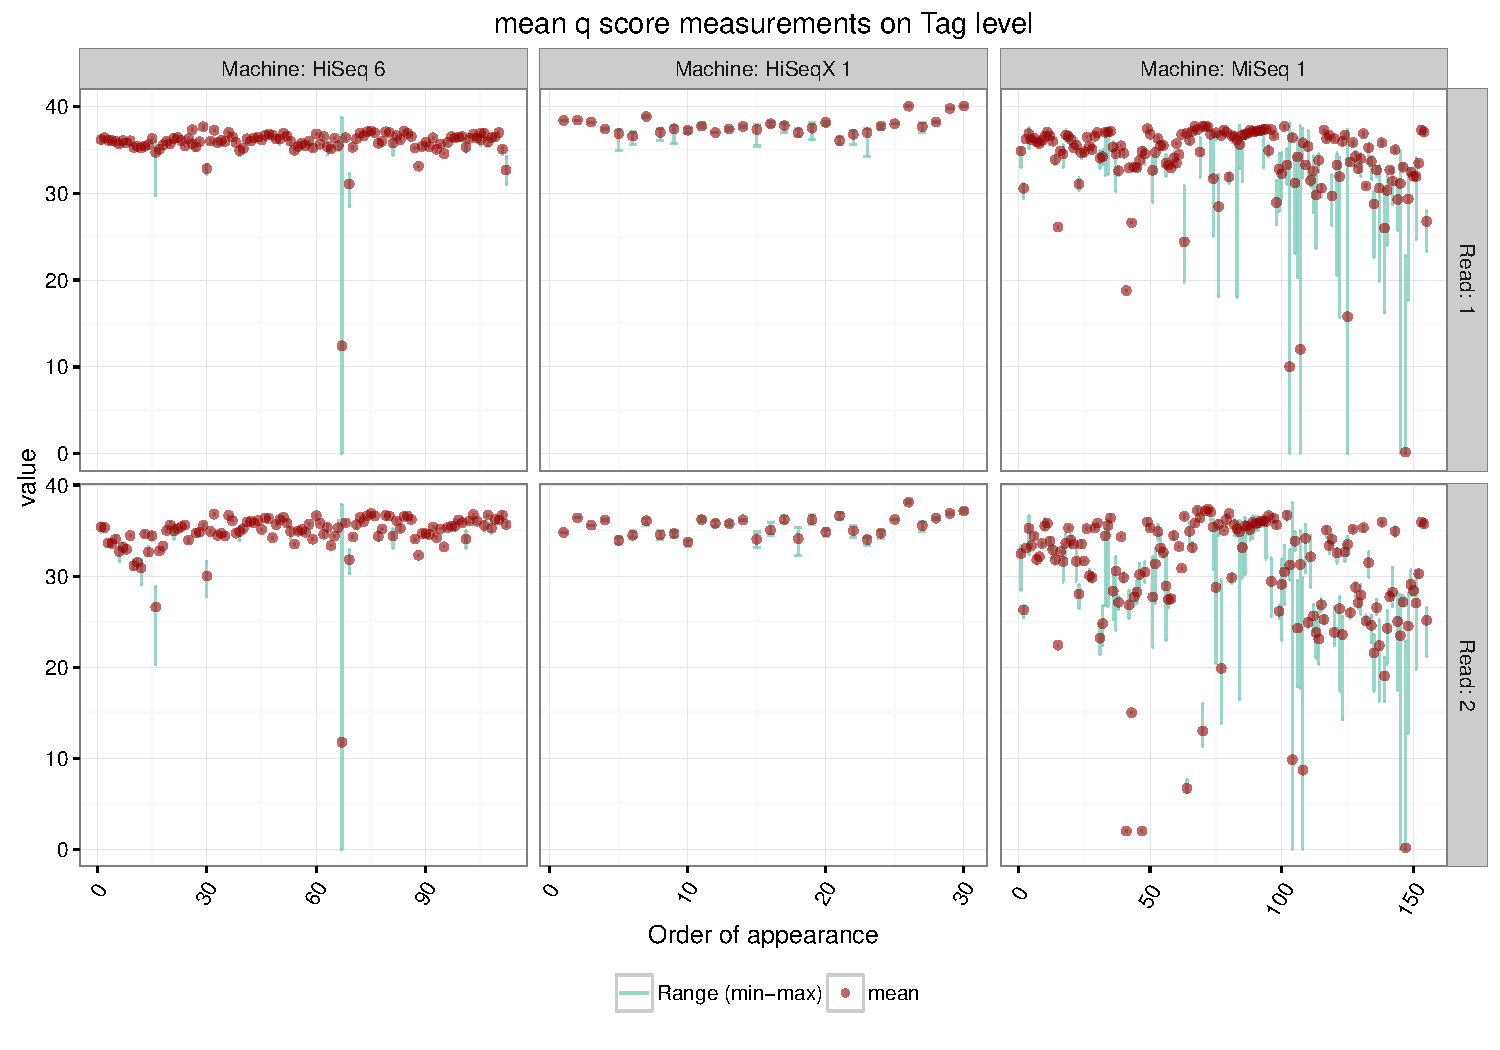
\includegraphics[scale=0.45]{EDA/figure/TagLevelTS-1.pdf} 
\end{center}
\end{frame}

\begin{frame}{Exploratory data analysis}{Tag level - \%data $>$ q30 and  tag error (HiSeq 6)}
\begin{center}
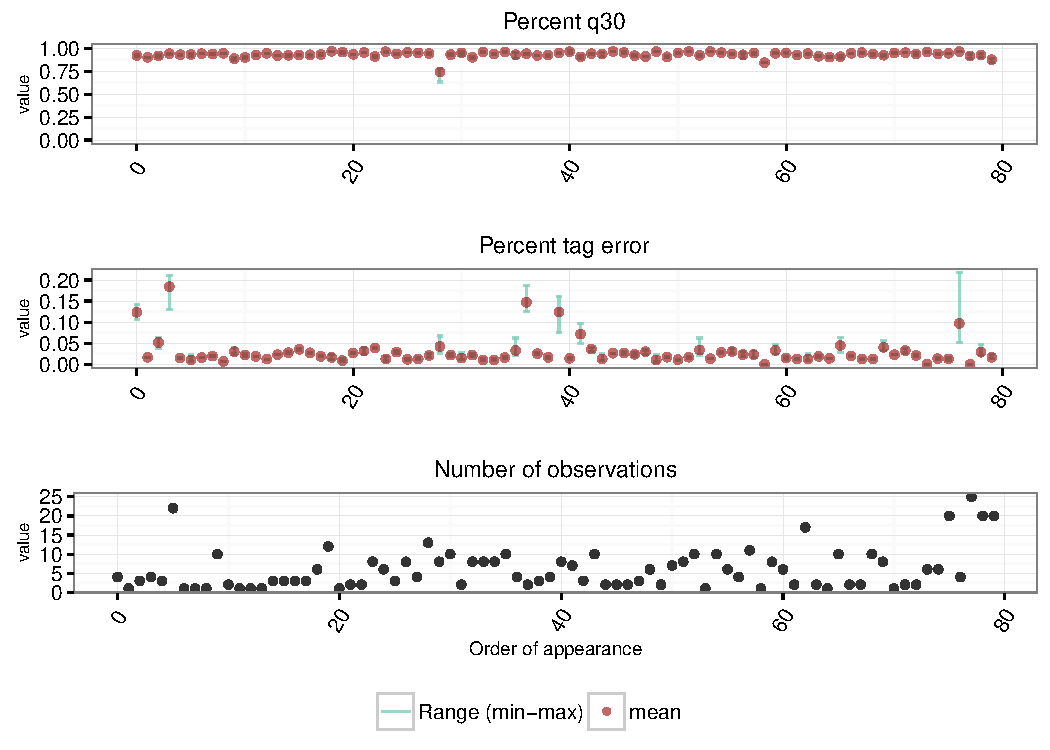
\includegraphics[scale=0.68]{EDA/figure/HiSeq6Comb-1.pdf} 
\end{center}
\end{frame}

\begin{frame}{Exploratory data analysis}{Read level - Correlation (HiSeq 6)}
\begin{center}
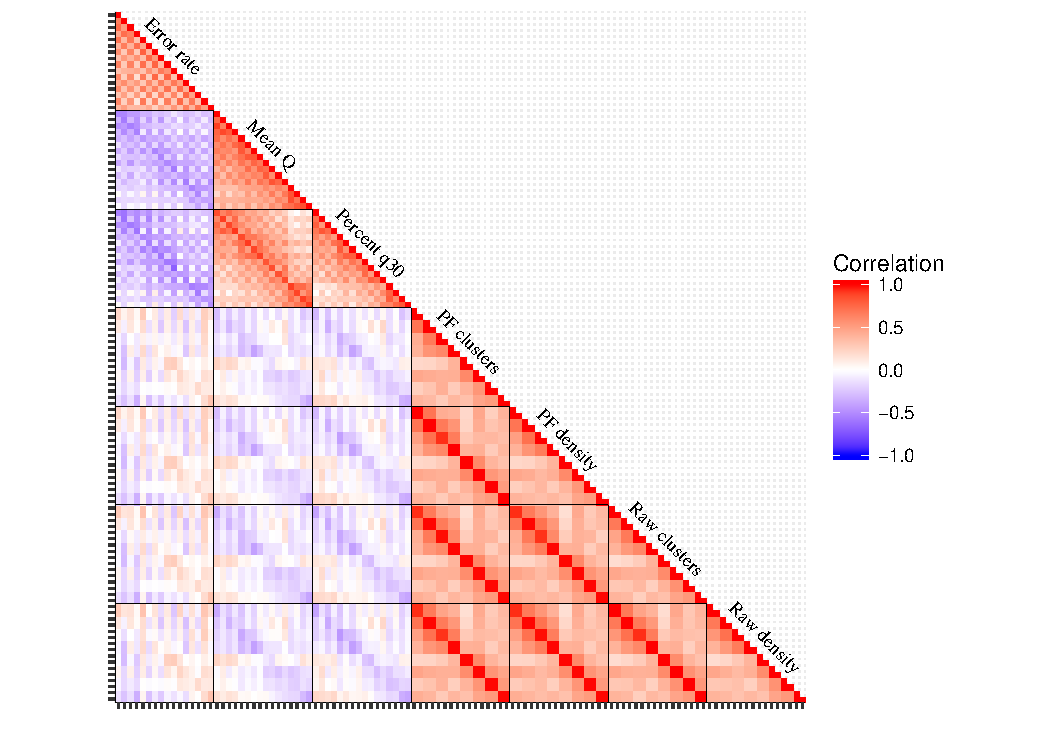
\includegraphics[scale=0.5, trim = 0mm 10mm 0mm 0mm, clip,]{EDA/figure/ReadlvlCor-1.pdf} 
\end{center}
\end{frame}

\begin{frame}{Exploratory data analysis}{Tag level results}
\begin{itemize}
\item Tag level has uneven number of observations in each lane/read. Sometimes one on each read/lane and sometimes up to 40+ $\rightarrow$ complicates things.
\item percent tag error is sometimes measured 0 (No PhiX in flowcell?) which also complicates things 
\item MiSeq machines will be hard (!) to profile and HiSeqX machines have small amount of data
\item Large variation inside flowcells.
\item Would like to but can not monitor Tag level -  uneven number of observations in each flowcell.
\item Aggregating to a flowcell level is not good enough, remove to much variation!
\end{itemize}
Solution: use read level measurements to monitor the machines and aggregate possible variables from tag to read level.
\end{frame}

\begin{frame}{Solution: Statistical process control (SPC)}
\begin{itemize}
\item A ''easy'' yet very powerful way to perform sequential hypothesis tests. Used in finance, food industry, production processes, monitoring patients in hospitals  
\item A lot of research have been put into the subject, though most under the assumption of normality
\item Pick a set of charts (models) which can be used to detect anomalies, trends and odd behaviours. One for estimation of the time the shift occurred.
\end{itemize}
\textit{Assumption: Transformed data follows a multivariate normal distribution.}
\end{frame}

\begin{frame}{Models}
Suggested solution in the SPC framework: \\
\begin{itemize}
\item Model for transient changes (anomalies): Hotellings $T^2$ 
\item Model for persistent changes (trends/maintenance, both mean and covariance): MCUSUM
\item Model for estimating changepoint: Will be thought of as a nonlinear optimization problem
\end{itemize}
\end{frame}

\begin{frame}{Hotelling's $T^2$}
Based on the statistical distance, let $\mathbf{X}_t$ represent new quality control data
$$
T^2_{t} = (\mathbf{X}_t-\hat{\boldsymbol{\mu}}_0)'\widehat{\boldsymbol{\Sigma}}^{-1}_0(\mathbf{X}_t-\hat{\boldsymbol{\mu}}_0)
$$ 
where $\hat{\boldsymbol{\mu}}_0$, $\widehat{\boldsymbol{\Sigma}}_0$ estimated from a train set of size $M$. Let $p$ be number of variables. If
$$
 T^2_{t} > \frac{p(M-1)(M+1)}{(M-p)M} F_{1-\alpha,p,M-p} \rightarrow ALARM
$$
$F_{1-\alpha,p,M-p}$ is the $1-\alpha$ percentile of F-distribution. 
\end{frame}

\begin{frame}{MCUSUM: A VERY brief introduction. }
Let $\mathbf{S}_0=\mathbf{0}$, and consider the following system
\begin{align*}
&C_t=\sqrt{(\mathbf{S}_{t-1}+\mathbf{X}_t-\hat{\boldsymbol{\mu}}_0)'\widehat{\boldsymbol{\Sigma}}^{-1}_0
(\mathbf{S}_{t-1}+\mathbf{X}_t-\hat{\boldsymbol{\mu}}_0)} &\\
\text{if} &\; C_t \leq k &\\
&\mathbf{S}_t = \mathbf{0}& \\
\text{else} &&\\
&\mathbf{S}_t = (\mathbf{S}_{t-1}+\mathbf{X}_t-\hat{\boldsymbol{\mu}}_0)(1-k/C_t)&
\end{align*}
Then $Y_t=\sqrt{\mathbf{S}_t'\widehat{\boldsymbol{\Sigma}}^{-1}_0 \mathbf{S}_t}>h \: \rightarrow ALARM$. $h$ connected to type 1 error, $k$ connected to what size of shifts we are interested in.
 
MCUSUM accumulates evidence on data which does not follow machines profile.
 How do we pick $k,h$? Pick type 1 error then use monte carlo simulation!
\end{frame}

\begin{frame}{Chain of models}
\begin{center}
\begin{figure}
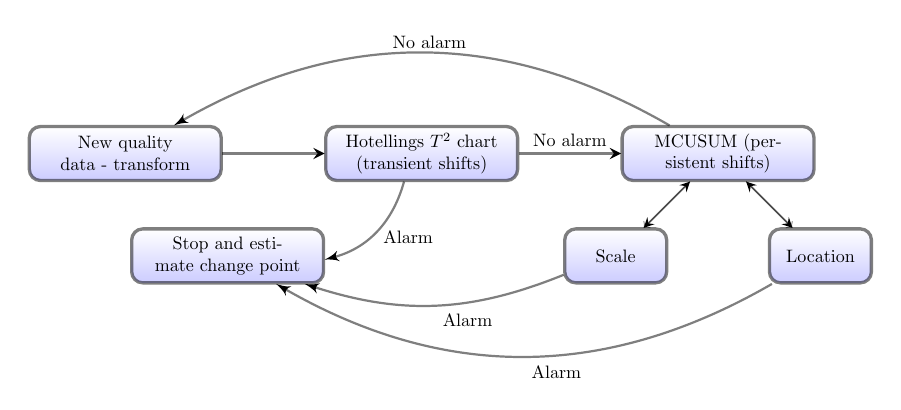
\begin{tikzpicture}[scale=0.65, transform shape,
	->,
	node distance=2cm,
	start chain=going right,
    Nice/.style={rectangle, 
    rounded corners, 
    draw=black, very thick,
    text width=5em, 
    minimum height=3em, 
    text centered, 
    on chain,
    top color=white, 
    bottom color=blue!20},
    line/.style={draw, thick, -latex'}
	every join/.style={->, thick,shorten >=1pt}
	fill opacity=.9,
	draw opacity=.5
	]
  \node [punktchain] (NewDat) {New quality data - transform};
  \node [punktchain] (Hot) {Hotellings $T^2$ chart (transient shifts)};
  \node [punktchain] (MCUSUM) {MCUSUM (persistent shifts)}
    child {node[Nice,below of = MCUSUM] (loc) {Location}}
    	child {node[Nice,below of = MCUSUM, xshift=-4cm] (scal) {Scale}};
  \draw [semithick, <->,>=stealth] (MCUSUM) -- (loc);
  \draw [semithick, <->,>=stealth] (MCUSUM) -- (scal);
  \node [punktchain, below of = NewDat] (Alarm) {Stop and estimate change point};
  \draw [arrow] (NewDat) -- (Hot);
  \draw [arrow] (Hot) -- node[anchor=south] {No alarm} (MCUSUM);
  \path [draw,thick,-latex',every node/.style={inner sep=1pt}] 
  		(Hot) edge [bend left=30] node[anchor=west, yshift=-0.1cm, xshift=0.1cm] {Alarm} (Alarm);
  \path[draw,thick,-latex',every node/.style={inner sep=1pt}]
  	    (loc) edge [bend left=30] node[right=1mm,yshift=-0.3cm] {Alarm} (Alarm);
  \path[draw,thick,-latex',every node/.style={inner sep=1pt}]
  	    (scal) edge [bend left=20] node[right=1mm,yshift=-0.3cm] {Alarm} (Alarm);
  \path[draw,thick,-latex']
  		(MCUSUM) edge [bend right=30] node[right=1mm, yshift=0.2cm, xshift=-.8cm] {No alarm} (NewDat);
\end{tikzpicture}
\end{figure}
\end{center}
\end{frame}

\begin{frame}{Results}
Done:
\begin{itemize}
\item Hotelling's $T^2$ chart
\item MCUSUM for location (mean)
\end{itemize}
In progress:
\begin{itemize}
\item Run MCUSUM for scale, no change in the algorithm needed only a lot of matrix multiplication and then re-run the whole thing.
\item The change-point estimation (for scale have not found theory on it) 
\item Even more simulations!
\end{itemize}
\end{frame}

\begin{frame}{Results: A tailored example}
Step for constructing the Hotelling and MCUSUM models used in this example.
\begin{enumerate}
\item Find a good profile for the machine (train set: HiSeq 6, v4-type, run cycles 126)
\item Estimate the parameters in model 
\item Use simulations to find parameters $h,k$.
\end{enumerate}
Use data which where not included in training as a test set. Can the models detect any change?

\textit{Disclaimer:} Data is not sequential $\rightarrow$ ruins the point somewhat, hence a tailored example.
\end{frame}


\begin{frame}{A tailored example: Hotelling's $T^2$}
\begin{center}
 \includegraphics[scale=0.5]{../../HotellingT2.pdf} 
\end{center}
\end{frame}

\begin{frame}{A tailored example: MCUSUM}
\begin{center}
\includegraphics[scale=0.5]{../../MCUSUM.pdf}
\end{center}
\end{frame}

\begin{frame}{Issues?}
\begin{itemize}
\item Sample size decreases a lot when stratifying on run-setting. Power goes down, estimation becomes more complicated etc. 
\item Very often n $<$ p. Train set sample size $\approx 75$, variables $\approx$ 110. Solution: Use PCA or some other sort for reduction technique.
\item Can we safely create a profile for a machine on a given run-setting? What about all the different run-settings each machine has? How can we deal with these issues?
\item Data really Normally distributed? Hypothesis tests $\rightarrow$ 2/3 says Yes. (p-value close to significance level...)
\item Non-parametric solutions exists but comes with odd assumptions and/or no clear theory of estimation of parameters and expectations. These methods need LOTS of data!
\item Takes a lot of time to approximate expectations (find parameters in models)! Approx. 1 day in C++ (R extension) to run simulations
\end{itemize}
\end{frame}

\end{document}